\documentclass[12pt]{article}
\usepackage[utf8]{inputenc}
\usepackage[russian]{babel}
\usepackage{graphicx}
\usepackage{listings}
\usepackage{indentfirst}
\usepackage{color}
\usepackage{multirow}
\usepackage{amsmath}
\usepackage{bm}

\definecolor{dkgreen}{rgb}{0,0.6,0}
\definecolor{gray}{rgb}{0.5,0.5,0.5}
\definecolor{ltgray}{rgb}{0.95,0.95,0.95}
\definecolor{mauve}{rgb}{0.58,0,0.82}
\newcommand{\rot}{\mathop{\rm rot}\nolimits}
\renewcommand{\lstlistingname}{Листинг}
\lstset{ %
  language=Python,                % the language of the code
  basicstyle=\footnotesize\ttfamily,           % the size of the fonts that are used for the code
%  numbers=left,                   % where to put the line-numbers
%  numberstyle=\tiny\color{gray},  % the style that is used for the line-numbers
%  stepnumber=2,                   % the step between two line-numbers. If it's 1, each line 
                                  % will be numbered
%  numbersep=5pt,                  % how far the line-numbers are from the code
  backgroundcolor=\color{ltgray},      % choose the background color. You must add \usepackage{color}
  showspaces=false,               % show spaces adding particular underscores
  showstringspaces=false,         % underline spaces within strings
  showtabs=false,                 % show tabs within strings adding particular underscores
  %frame=single,                   % adds a frame around the code
  rulecolor=\color{black},        % if not set, the frame-color may be changed on line-breaks within not-black text (e.g. comments (green here))
  columns=fixed,
  tabsize=2,                      % sets default tabsize to 2 spaces
  captionpos=b,                   % sets the caption-position to bottom
  breaklines=true,                % sets automatic line breaking
  breakatwhitespace=false,        % sets if automatic breaks should only happen at whitespace
%  caption=Valalala,                   % show the filename of files included with \lstinputlisting;
                                  % also try caption instead of title
  keywordstyle=\color{blue},          % keyword style
  commentstyle=\color{gray},       % comment style
  stringstyle=\color{dkgreen},         % string literal style
  escapeinside={\%*}{*)},            % if you want to add LaTeX within your code
  morekeywords={*,...},              % if you want to add more keywords to the set
  deletekeywords={...}              % if you want to delete keywords from the given language
}


\title{Численное сравнение схем расщепления для нестационарного уравнения Стокса}
\author{Борисов В.С.}

\begin{document}

\maketitle

\section{Задача}
Рассматривается применение схем расщепления для нестационарного уравнения Стокса, которое описывает течение сильно вязкой несжимаемой жидкости. Исходная система связывает в одном уравнение переменные скорости и давления, что при использовании метода конечных элементов, увеличивает количество одновременно решаемых неизвестных. Путем расщепления неизвестные скорости и давления вычисляются по отдельности, то есть вместо составления матрицы включающей обе неизвестные, используются меньшие размером матрицы. При этом изменяется погрешность и время вычисления численного решения.

Нестационарное уравнение Стокса описывает течение несжимаемой жидкости в области $\Omega$ с границей $\partial \Omega$:
\begin{equation}
\begin{split}
\frac{\partial {\bm u}({\bm x}, t)}{\partial t} -\Delta {\bm u}({\bm x}, t) + \nabla p({\bm x}, t) &= {\bm f}({\bm x}, t), \\
\nabla\cdot{\bm u}({\bm x}, t) &= 0, 
\end{split}
\quad {\bm x} \in \Omega, \quad 0<t \leq T,
\end{equation} 

$$
{\bm u(\bm x, t)} = {\bm g}({\bm x}, t), \quad {\bm x} \in \partial \Omega,
$$
$$
{\bm u(\bm x, 0)} = {\bm u_0}({\bm x}), \quad {\bm x} \in \Omega,
$$
где ${\bm u}({\bm x}, t)$ - скорость, $p({\bm x}, t)$ - давление и ${\bm f}({\bm x}, t)$ - внутренний источник движения. В двумерном случае ${\bm x}=(x_1, x_2)$.

Рассматривается тестовая двумерная задача о течении в каверне с подвижной верхней границей. Подвижная верхняя граница означает, что вектор скорости на ней имеет ненулевое значение. Задача решается в безразмерных величинах на единичном квадрате $\Omega$ (рис. \ref{fg:cavity}), c границей $\partial \Omega=\Gamma_1 \cup \Gamma_2$, где на верхней границе $\Gamma_1$ скорость принимает значения ${\bm u}=(1, 0, t)$, в остальной части $\Gamma_2$ поставлено условие ${\bm u}=(0, 0, t)$ для $0<t \leq T$. Внутренние источники отсутствуют - правая часть равна нулю. Таким образом, решаемая задача имеет следующую постановку:
\begin{equation}
\begin{split}
\frac{\partial {\bm u}({\bm x}, t)}{\partial t} -\Delta {\bm u}({\bm x}, t) + \nabla p({\bm x}, t) &= 0, \\
\nabla\cdot{\bm u}({\bm x}, t) &= 0, 
\end{split}
\quad {\bm x} \in \Omega, \quad 0<t \leq T,
\label{eq:scheme-main}
\end{equation} 
с граничными условиями:
\begin{equation}
\begin{split}
{\bm u(\bm x, t)} &= (1, 0, t), \quad {\bm x} \in \Gamma_1,  \\
{\bm u(\bm x, t)} &= (0, 0, t), \quad {\bm x} \in \Gamma_2, \\
\end{split}
\quad 0<t \leq T,
\label{eq:scheme-boundary}
\end{equation} 
и начальным условием:
\begin{equation}
{\bm u(\bm x, 0)} = (0, 0), \quad {\bm x} \in \Omega.
\label{eq:scheme-start}
\end{equation}

\begin{figure}
	\begin{center}
		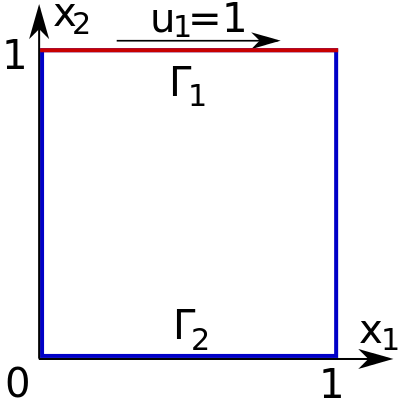
\includegraphics[width=200px]{pics/cavity400}
		\caption{Тестовая область с подвижной верхней границей.}
		\label{fg:cavity}
	\end{center}
\end{figure}


%\section{Численная реализация}
%Система уравнений (\ref{eq:scheme-main}) приводится к вариационной постановке.

\section{Вариационная постановка}
Для решения задачи, уравнение (\ref{eq:scheme-main}) приводится к вариационной постановке \cite{fenicsbook-2012}. Введем следующие функциональные пространства используя пространства Соболева ($H$) и Гильберта ($L^2$).
$$
V=\{ ({\bm u}, p) : \, {\bm u} \in H(div, \Omega), \, p \in L^2(\Omega) \},
$$
$$
\hat V=\{ ({\bm v}, q) : \, {\bm v} \in H(div, \Omega), \, q \in L^2(\Omega), \, {\bm v}|_{\partial \Omega}=0 \}.
$$
Умножим уравнения (\ref{eq:scheme-main}) с неизвестными функциями ${\bm u}, p \in V$  на тестовые функции ${\bm v}, q \in \hat V$ соответственно, и возьмем интеграл по $\Omega$:
$$
\int_{\Omega} \frac{\partial {\bm u}}{\partial t} \cdot {\bm v} \,dx - \int_{\Omega} \Delta {\bm u} \cdot {\bm v} \,dx + \int_{\Omega} \nabla p \cdot {\bm v} \,dx = 0,
$$
$$
\int_{\Omega} (\nabla \cdot {\bm u}) \cdot q \,dx = 0.
$$
Используя формулу Грина, преобразуем оператор Лапласа:
$$
\int_{\Omega} \frac{\partial {\bm u}}{\partial t} \cdot {\bm v} \,dx + \int_{\Omega} \nabla {\bm u} \cdot \nabla {\bm v} \,dx - \int_{\partial \Omega} \frac{\partial {\bm u}}{\partial {\bm n}} \cdot {\bm v} \,dS + \int_{\Omega} \nabla p \cdot {\bm v} \,dx = 0,
$$
здесь интеграл по $\partial \Omega$ равен нулю, т.к. функция ${\bm v} | _ {\partial \Omega} = 0$. Общая вариационная постановка в смешанном пространстве $\hat V$ выглядит следующим образом:
$$
\int_{\Omega} \frac{\partial {\bm u}}{\partial t} \cdot {\bm v} \,dx + \int_{\Omega} \nabla {\bm u} \cdot \nabla {\bm v} \,dx + \int_{\Omega} \nabla p \cdot {\bm v} \,dx + \int_{\Omega} (\nabla \cdot {\bm u}) \cdot q \,dx = 0.
$$
Расщепление производится по временному слагаемому из уравнения (\ref{eq:scheme-main}). Для каждой схемы строится отдельная вариационная постановка с использованием уже введенных пространств, но принцип преобразования оператора Лапласа и избавление от интеграла по границе сохраняется.


\section{Схемы}
%Для решения использовано сочетание конечных элементов Тейлора-Худа.
%Для применения схемы расщепления исходная система уравнений (\ref{eq:scheme-main}) приводится к операторному виду:
%$$
%\frac{\partial {\bm u}}{\partial t} + {\cal N}{\bm u} + {\cal P}{\bm u} = 0,
%$$
%где операторы 
%$$
%{\cal N}{\bm u} = -\Delta {\bm u},
%$$
%$$
%{\cal P}{\bm u} = \nabla p,
%$$ 
%при условии 
%\begin{equation} \label{eq:scheme-zerodiv}
%\nabla\cdot {\bm u} = 0.
%\end{equation}
%%Расписать свойства операторов
%Свойства этих операторов позволяют применять следующие схемы расщепления:
%\begin{itemize}
%\item схема Дугласа-Рекфорда,
%\item схема Письмана-Рекфорда,
%\item покомпонентная схема.
%\end{itemize}
%Для сравнения задача решается также с использованием следующих схем без расщепления:
%\begin{itemize}
%\item чисто неявная схема,
%\item схема Кранка-Николсона.
%\end{itemize}
%%Расписать про tau n
%Введем дискретные переменные ${\bm y}$ и $e$ для ${\bm u}$ и $p$ соответственно. Шаг по времени обозначается как $\tau$.
Схемы расщепления применяются для аппроксимации производной по времени. Введем равномерный шаг по времени $\tau$. Исходное уравнение разделяется на два уравнения путем введения промежуточного значения ${\bm u}^*={\bm u}_h^{n+\frac{1}{2}}$ между временными слоями ${\bm u}_h^n$ и ${\bm u}_h^{n+1}$.
\paragraph{Схема Дугласа-Рекфорда.} Особенность разбиения состоит в уменьшении размера матрицы для СЛАУ. Вместо составления единого смешанного пространства переменных скорости и давления, вычисления проводятся для скорости и давления по отдельности \cite{vabishchevich-1999}. 
\begin{equation} \label{eq:scheme-douglas-1}
\frac{{\bm u}^{*}-{\bm u}_h^n}{\tau} - \Delta {\bm u}^{*}+{\nabla}p_h^n=0,
\end{equation}
\begin{equation} \label{eq:scheme-douglas-2}
\frac{{\bm u}_h^{n+1}-{\bm u}_h^n}{\tau} - \Delta {\bm u}^{*}+{\nabla}p_h^{n+1}=0,
\end{equation}
\begin{equation} \label{eq:scheme-douglas-3}
\nabla \cdot {\bm u}_h^n = 0.
\end{equation}
Вычисление ${\bm u}_h^{n+1}$ и $p_h^{n+1}$ происходит в несколько этапов:
\begin{enumerate}
\item 
Сперва вычисляется ${\bm u}^*$, для этого умножим уравнение (\ref{eq:scheme-douglas-1}) на функцию $\bm v$ и возьмем интеграл по $\Omega$, используя формулу Грина для преобразования оператора Лапласа:
$$
\frac{1}{\tau}\int_{\Omega} {\bm u}^*\cdot {\bm v} \,dx + \int_{\Omega} \nabla {\bm u}^* \cdot \nabla {\bm v} \,dx = -\int_{\Omega} {\bm v} \cdot \nabla p_h^{n}\, dx + \frac{1}{\tau} \int_{\Omega} {\bm u}_h^{n} \cdot {\bm v} \,dx.
$$
Решается линейная задача $a({\bm v}, {\bm u}^*) = L({\bm v})$, где
$$
a({\bm v}, {\bm u}) = \frac{1}{\tau}\int_{\Omega} {\bm u}^*\cdot {\bm v} \,dx + \int_{\Omega} \nabla {\bm u}^* \cdot \nabla {\bm v} \,dx,
$$
$$
L({\bm v}) = -\int_{\Omega} {\bm v} \cdot \nabla p_h^{n} \,dx + \frac{1}{\tau} \int_{\Omega} {\bm u}_h^{n} \cdot {\bm v} \,dx;
$$
\item 
Вычитаем из (\ref{eq:scheme-douglas-2}) уравнение (\ref{eq:scheme-douglas-1}):
\begin{equation} \label{eq:scheme-douglas-1}
\frac{{\bm u}_h^{n+1}-{\bm u}^*}{\tau} + {\nabla}(p_h^{n+1} - p_h^n )=0.
\end{equation}
Применяем дивергенцию, из равенства ({\ref{eq:scheme-douglas-3}}) первое слагаемое обнуляется:
$$
\Delta \gamma = \frac{1}{\tau} \nabla \cdot u^{*},
$$
где 
$$
\gamma = p_h^{n+1}-p_h^n.
$$
Вычисляем $\gamma$ из:
$$
a(q, \gamma) = -\int_{\Omega} \nabla \gamma \nabla q \,dx,
$$
$$
L(q) = \frac{1}{\tau} \int_{\Omega} \nabla \cdot {\bm u}^* q \,dx;
$$
\item 
Вычисляем ${\bm u}_h^{n+1}$ из (\ref{eq:scheme-douglas-2}):
$$
a({\bm v}, {\bm u}_h^{n+1}) = \frac{1}{\tau} \int_{\Omega} {\bm u}_h^{n+1} \cdot {\bm v}\,dx,
$$
$$
L({\bm v}) = \frac{1}{\tau} \int_{\Omega} {\bm u}^* \cdot v \,dx - \int_{\Omega} \nabla \gamma \cdot {\bm v} \,dx;
$$
\item 
Находим $p_h^{n+1}$:
$$
a(q, p) = \int_{\Omega} p_h^{n+1} q\,dx,
$$
$$
L(q) = \int_{\Omega} (\gamma + p_h^n) q\,dx.
$$
\end{enumerate}

%Вычисления проводится в три этапа:
%\begin{enumerate}
%\item Вычисляем ${\bm y}^{n+\frac{1}{2}}$ из первого уравнения;
%\item Вычитаем из (\ref{eq:scheme-douglas-2}) уравнение (\ref{eq:scheme-douglas-1}). Получаем уравнение:
%\begin{equation} \label{eq:scheme-douglas-add}
%\frac{{\bm y}^{n+1}-{\bm y}^{n+\frac{1}{2}}}{\tau} + {\cal P}({\bm y}^{n+1}-{\bm y}^{n})=0,
%\end{equation}
%где оператор ${\cal P}$ на самом деле работает с давлением $e$. Возьмем дивергенцию от (\ref{eq:scheme-douglas-add}). Используя условие (\ref{eq:scheme-zerodiv}) избавляемся от ${\bm y}^{n+1}$ и вычисляем $\gamma = e^{n+1}-e^{n}$.
%\item Подставив $\gamma$ в (\ref{eq:scheme-douglas-add}) явно вычислим ${\bm y}^{n+1}$.
%\end{enumerate}
\paragraph{Схема Письмана-Рекфорда.} Особенностью схемы является меньший шаг по времени $\tau/2$ и другое использование промежуточного ${\bm u}^*$. Вычисления происходит аналогично схеме Дугласа-Рекфорда.
$$
\frac{{\bm u}_h^{*}-{\bm u}_h^n}{\tau/2} - \Delta {\bm u}^{*}+\nabla p_h^n=0,
$$
$$
\frac{{\bm u}^{n+1}-{\bm u}^{*}}{\tau/2} - \Delta {\bm u}^{*}+\nabla p_h^{n+1}=0,
$$
$$
\nabla \cdot {\bm u}_h^n = 0.
$$

\paragraph{Покомпонентная схема.} Расщепление происходит по физическим компонентам. Так в первое уравнение для скорости, а второе для давления. Вычисления происходит аналогично схеме Дугласа-Рекфорда.
$$
\frac{{\bm u}_h^{*}-{\bm u}_h^n}{\tau} - \Delta{\bm u}^{*}=0,
$$
$$
\frac{{\bm u}_h^{n+1}-{\bm u}_h^{*}}{\tau} + \nabla p_h^{n+1}=0,
$$
$$
\nabla \cdot {\bm u}_h^n = 0.
$$


\paragraph{Чисто неявная схема.} Чисто неявная схема приведена для сравнения точности со схемами расщепления.
$$
\frac{{\bm u}_h^{n+1}-{\bm u}_h^n}{\tau} - \Delta {\bm u}_h^{n+1}+\nabla p_h^{n+1} = 0,
$$
$$
\nabla \cdot {\bm u}_h^{n+1} = 0.
$$
\paragraph{Схема Кранка-Николсона.} Схема приведена для сравнения точности со схемами расщепления.
$$
\frac{{\bm u}_h^{n+1}-{\bm u}_h^n}{\tau} - \Delta \frac{{\bm u}_h^{n+1}+{\bm u}_h^n}{2}+\nabla \frac{p_h^{n+1}+p_h^n}{2}=0,
$$
$$
\nabla \cdot \frac{{\bm u}_h^{n+1}+{\bm u}_h^{n}}{2}=0.
$$

\section{Результат}
Вычисления проводились на сетках размером $N = 20, 40, 80, 160$, где $N$ это количество узлов на ребре единичного квадрата. Шаг по времени $\tau = 0.01, 0.005, 0.0025$. Для сравнения нормы погрешности вычисляется ``псевдоточное'' решение ${\bm u}_{ex}^n$, чисто неявная схема, на сетке размером $N=200$ и $\tau=0.00125$.
Вычисление нормы $L_2(\Omega)$ погрешности $\epsilon^n$ для временного слоя $n$:
$$
\epsilon^n = \sqrt{\int_{\Omega} ({\bm u}_h^n - {\bm u}_{ex}^n )^2 \, dx}.
$$

Графики на рис. \ref{fg:scheme-L2-1} - \ref{fg:scheme-L2-4} показывают норму погрешности $L_2(\Omega)$. По оси X временные слои, по оси Y норма. Обозначения схем на рисунках:
\begin{itemize}
\item cn - схема Кранка-Николсона,
\item dr - схема Дугласа-Рекфорда,
\item im - чисто неявная схема,
\item ct - покомпонентная схема,
\item pr - схема Письмана-Рекфорда.
\end{itemize}
Схемы расщепления проигрывают по точности чисто неявной и Кранка-Николсона, при этом  схема Письмена-Рекфорда неустойчива на сетке $N=20$ независимо от $\tau$. При увеличении размера сетки схема Дугласа-Рекфорда заметно приближается к неявной и Кранка-Николсона.

График на рис. \ref{fg:scheme-time} показывает что время вычисления по схемам расщепления быстрее чем по неявной и Кранка-Николсона. Таким образом схема Дугласа-Рекфорда наиболее предпочтительная для решения задач данного типа.

\begin{figure}
	\begin{center}
		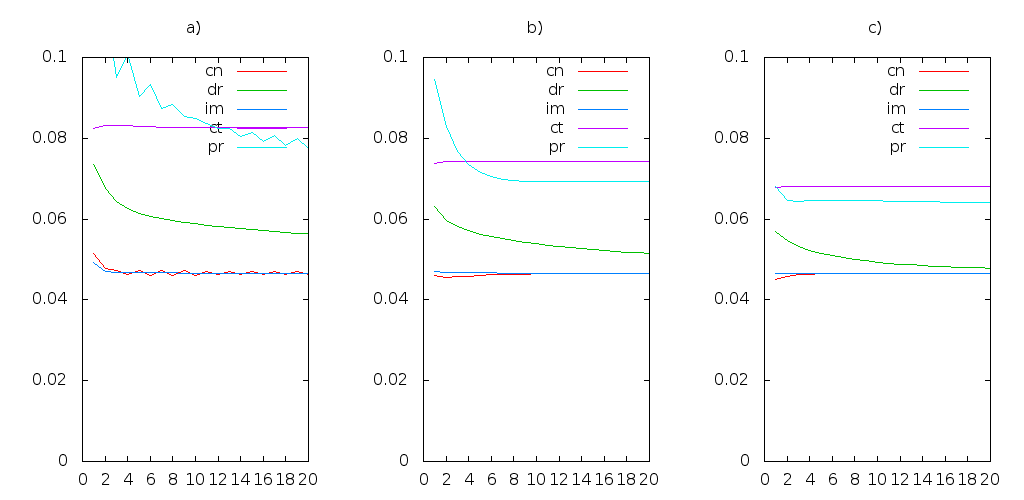
\includegraphics[width=400px]{data160/error_1}
		\caption{Норма погрешности скорости в $L_2$ для $N=20$, a) $\tau=0.01$, b) $\tau=0.005$, c) $\tau=0.0025$.}
		\label{fg:scheme-L2-1}
	\end{center}
\end{figure}

\begin{figure}
	\begin{center}
		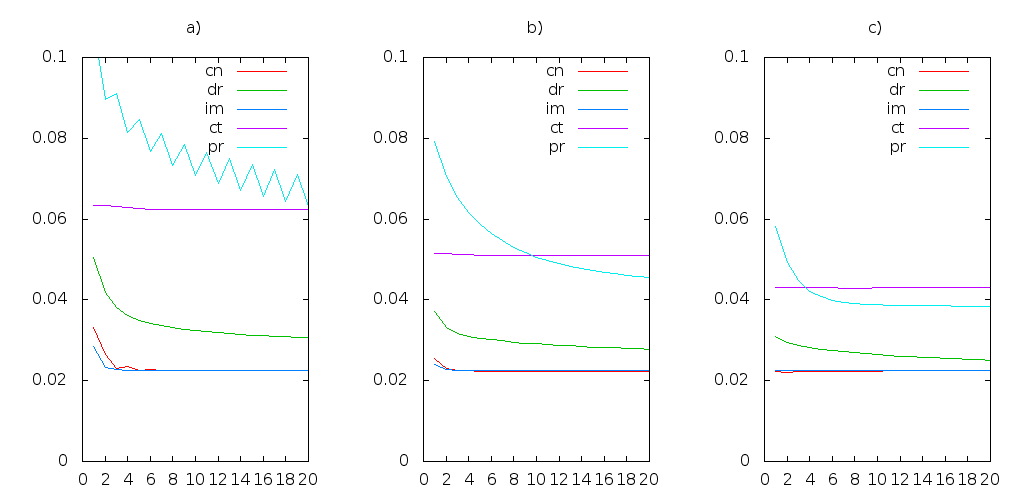
\includegraphics[width=400px]{data160/error_2}
		\caption{Норма погрешности скорости в $L_2$ для $N=40$, a) $\tau=0.01$, b) $\tau=0.005$, c) $\tau=0.0025$.}
		\label{fg:scheme-L2-2}
	\end{center}
\end{figure}

\begin{figure}
	\begin{center}
		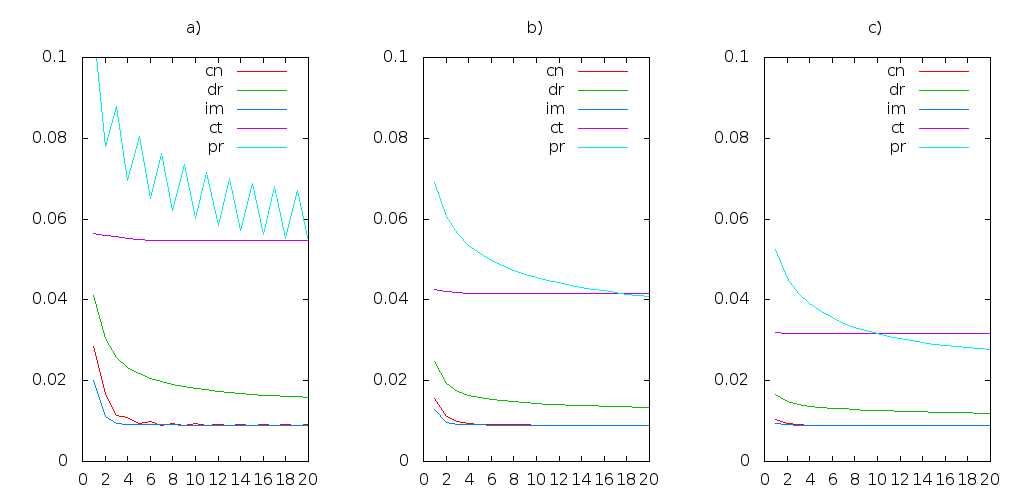
\includegraphics[width=400px]{data160/error_3}
		\caption{Норма погрешности скорости в $L_2$ для $N=80$, a) $\tau=0.01$, b) $\tau=0.005$, c) $\tau=0.0025$.}
		\label{fg:scheme-L2-3}
	\end{center}
\end{figure}

\begin{figure}
	\begin{center}
		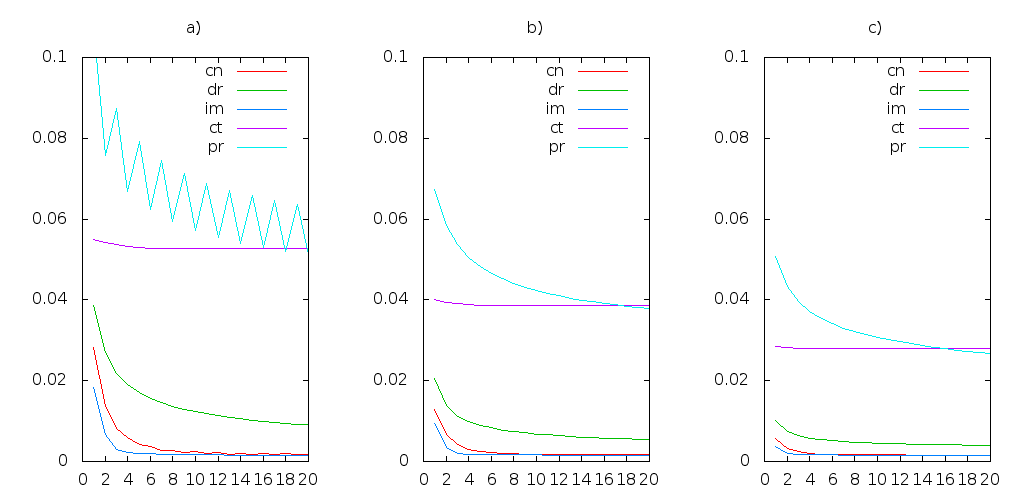
\includegraphics[width=400px]{data160/error_4}
		\caption{Норма погрешности скорости в $L_2$ для $N=160$, a) $\tau=0.01$, b) $\tau=0.005$, c) $\tau=0.0025$.}
		\label{fg:scheme-L2-4}
	\end{center}
\end{figure}

\begin{figure}
	\begin{center}
		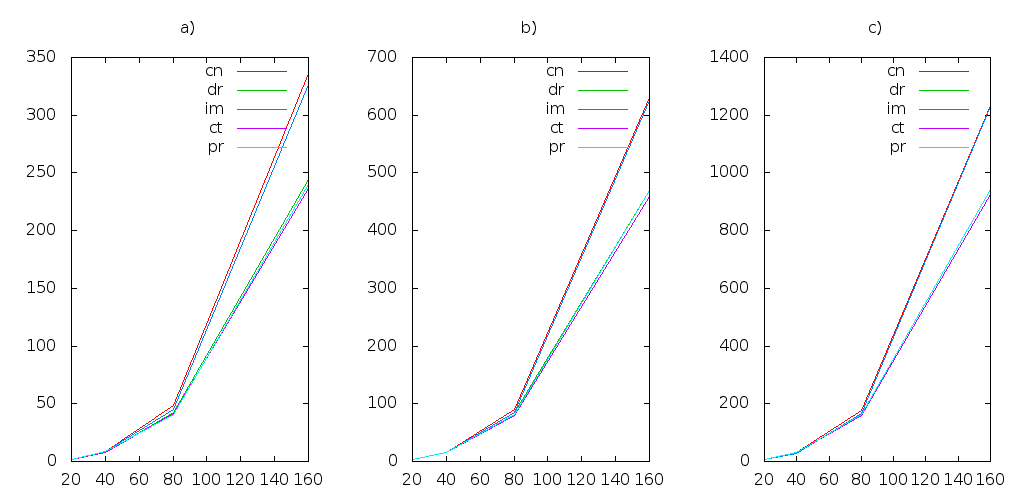
\includegraphics[width=400px]{data160/scheme-time}
		\caption{Время вычисления для a) $\tau=0.01$, b) $\tau=0.005$, c) $\tau=0.0025$.}
		\label{fg:scheme-time}
	\end{center}
\end{figure}

\begin{thebibliography}{9}
\bibitem{vabishchevich-1999} Самарский А.А., Вабищевич П.Н. Аддитивные схемы для задач математической физики. \newblock --- М.: Наука, 1999. 319~с.
\bibitem{fenicsbook-2012} Anders Logg, Kent-Andre Mardal, Garth Wells. Automated Solution of Differential Equations by the Finite Element Method. \newblock --- Berlin: Springer Berlin Heidelberg, 2012. 723~p.
\end{thebibliography}

\end{document}